%\NeedsTeXFormat{LaTeX2e}
%\listfiles
%\setcounter{errorcontextlines}{\maxdimen}
\documentclass[10pt,utf8, mainlanguage=english]{ufcd-info}

\usepackage[T1]{fontenc}
%\usepackage[xutf8]{inputenc}
\usepackage{graphicx}
\usepackage{rotating}
\usepackage{tabularx}
\usepackage{natbib}
\usepackage{color}
%\usepackage[final]{changes}
\usepackage[authormarkup=none, draft]{changes}
\usepackage[style=english]{csquotes}
\usepackage{fancyhdr}
\usepackage{hyperref}
\usepackage{nameref}
%\setlength{\headheight}{7.2pt}
\pagestyle{plain}
%\fancyhf{}
%\rhead{\today}
%\cfoot{\thepage}
\author{Rolf Würdemann, Julia Meier}


\title{API definitions for the FMF libs}
\date{\today}

\definechangesauthor[color=blue]{rw}
\definechangesauthor[color=orange]{jm}
\newcommand{\fret}[1]{{\texttt{#1}}}
\newcommand{\fcal}[2]{{\textbf{#1}}(\textit{#2})}
\newcommand{\fmfattr}[1]{{\textbf{#1}}}
\newcommand{\fmfobj}[1]{{\textbf{\textsf{#1}}}}
\newcommand{\rework}[1]{\textcolor{red}{TO BE REWORKED[} #1 \textcolor{red}{]}}

\begin{document}

\hyphenation{FMF-Table FMF-Me-ta-Sec-tion}

\maketitle
\thispagestyle{empty}

\section{Introduction}

Riede {\sl et al.} invented the \enquote{Full-Metadata Format} (FMF) in \cite{RiedeCPC181_2010}. The FMF is a self documenting, human readable data storage and interchange format for the so called \enquote{small science}. One of the outstanding features of the FMF is the definition of a structure which glues together data and metadata within one file while preserving the freedom of choice which metadata to store and how to arrange it. By this means it is optimized for the storage and interchange of tabular research data. There are implementations of the FMF as part of the data analysis software \enquote{Pyphant} and in basic libraries\footnote{See Appendix}. To provide easy access to the FMF, the idea of developing separate libraries providing full compliance to \cite{RiedeCPC181_2010} was born also in 2010. This report gives a textual overview of the objects and their application programming interface (API).

By the philosophy of the FMF, acquired data belongs to one of two types of objects: On one side the actual data, either measured, derived or calculated and on the other side the metadata, describing the data and circumstances of their acquisition and providing information for reference. This view on data is represented in the definition of the FMF. It contains sections holding the metadata, the corresponding object is further called \fmfobj{FMFMetaSection}. Afterwards the (usually) numerical data is stored in tables, the corresponding object is further called \fmfobj{FMFTable}. A third object which doesn't correspond directly to the data is the \fmfobj{FMFHeader} which holds information for data interchange and file representation such as encoding, field separator and comment character. The main object \fmfobj{FMF} can hold several \fmfobj{FMFMetaSection} and \fmfobj{FMFTable} objects, as well as it holds information on the FMF version for which it is generated and the compliance level as described below. As the compliance level is an inherent trait of the libraries internal handling of objects, that does not effect writing, it will not be written to a file.


\section{Compliance levels}
\label{sec:cls}

The FMF is a very powerful format for keeping data and metadata together. However, not every situation needs full functionality, especially consistency checks, and thus strict compliance to the definitions of data structures in \cite{RiedeCPC181_2010}. For an easier implementation, which also reflects the available amount of CPU power and memory, we have defined the following three compliance levels (CL):

\begin{itemize}
	\item {\bf CL 1:} Metadata and data definitions are stored as key-value pairs. Keys and values are stored as strings. Data are stored in their respective types and might be written to file using a specified formatter. There are no special fields for quantity, unit or uncernity. The only constraints checked are:
	\begin{itemize}
		\item Does the number of rows and columns match with the number stored in the {\sl no\_columns} and {\sl no\_rows} attributes of the corresponding \fmfobj{FMFTable} object
		\item The uniqueness of names of the \fmfobj{FMFMetaSection} objects belonging to  an \fmfobj{FMF} object and the uniqueness of keys within individual \fmfobj{FMFMetaSection} objects
		\item The existence of names and symbols of \fmfobj{FMFTable} objects as well as their uniqueness, if they are mandatory, and the uniqueness of keys in the data definitions within one \fmfobj{FMFTable} object
	\end{itemize}
	CL 1 is mainly meant for writing.
	\item {\bf CL 2:} In opposite to CL 1, values in \fmfobj{FMFMetaSections} are stored in their respective types. Dependencies, units, quantities and uncertainties are stored in separate attributes, but still stored as strings.
	In addition to the constraints checked by CL 1, the following constraints are checked:
		\begin{itemize}
		\item Matching of the dependencies in the definitions of \fmfobj{FMFTables},
		\item Compliance of the units with the unit definitions according to the specified FMF version
	\end{itemize}
	CL 2 is meant to give applications the possibility for easy processing.
	\item {\bf CL 3:} In addition to CL 2, quantities and units are stored in their respective types and in separate attributes which enable easy processing. In addition to CL 2, the following constraints are checked:
	 \begin{itemize}
		\item Matching of the units (if possible)
		\item Matching of the quantities (if possible)
	\end{itemize}
	CL 3 ensures full compliance to the definition of FMF in \cite{RiedeCPC181_2010}.
\end{itemize}

\section{Application Programming Interface (API)}\label{sec:API}
In the following the application programming interface (API) including attributes and public methods is defined. The first object defined is the \fmfobj{FMF}, which glues toghether the different sections and tables. Afterwards the API for the central objects is described in the order of \fmfobj{FMFMetaSection} and \fmfobj{FMFTable}.

Note that any FMF object is an ordered structure. \fmfobj{FMFMetasection}s and \fmfobj{FMFTable}s are added to an \fmfobj{FMF} in order of their initialization. Analogously global comments can be added before and after an \fmfobj{FMFMetasection} or \fmfobj{FMFTable}. Key-value pairs and comments appear in an \fmfobj{FMFMetasection} in the order they were added. This idea holds true also for \fmfobj{FMFTable}s. Although, due to the more complex structure, it is realized differently: For example, a comment added after a column appears in the data definitions after the definition of the column and not in the data part of the table. However, it still appears after the object after which it was added.

On errors, all methods should raise an exception. If this is impossible, a value corresponding to NULL in C should be returned for instantiators or a zero-element/false otherwise. The appropriate error-variables should be set with the error-code and message defined by the list of errors in the appendix.

\subsection{FMF}\label{subsec:FMF}

The \fmfobj{FMF} is the main object that corresponds to the entire FMF file. It is composed of \fmfobj{FMFMetaSection} objects holding the metadata and \fmfobj{FMFTable} objects holding the data, the \fmfobj{FMFHeader} and several additional attributes.

\subsubsection{Public Attributes:}
\begin{itemize}
	\item \fret{FMFHeader} \fmfattr{header}: The basic parameters for the file representation of FMF object
	\item \fret{FMFMetaSection[]} \fmfattr{meta\_sections}: A list containing the metadata sections of the FMF object
	\item \fret{FMFTable[]} \fmfattr{tables}: A list containing the tables with the actual data
	\item \fret{FMFComment[]} \fmfattr{global\_comments}: A list of global comments
	\item \fret{int} \fmfattr{compliance\_level}: Compliance level of FMF object
	\item \fret{int} \fmfattr{max\_compliance\_level}: Maximum compliance level supported by the library
	\item \fret{float} \fmfattr{version}: Version of FMF for which the current object was created
	\item \fret{float} \fmfattr{max\_version}: Maximum version supported by the library
\end{itemize}

\subsubsection{Public methods:}

\begin{itemize}
	\item \fret{FMF} \fcal{initialize}{}: Initializes the object. Returns the object itself on successfull initialization. \fmfattr{initialize} can be called either without any argument or with arguments \textit{title}, \textit{creator}, \textit{place}, \textit{created} and \textit{contact}. In the first case an empty \fmfobj{FMF} object is returned, in the latter a minimal valid \fmfobj{FMF} object with reference section defined by the input variables is returned. Because it is not defined in \cite{RiedeCPC181_2010}, \textit{contact} is optional in the latter case. This method might be called also by the language specific object initialization routines.

	\item \fret{FMFMetaSection} \fcal{set\_reference}{title, creator, place, created, contact}: Add the mandatory \enquote{*reference} section to an \fmfobj{FMF}. \textit{title}, \textit{creator}, \textit{place} and \textit{created} are mandatory, \textit{contact} is optional. If the section \enquote{*reference} already exists its values will be changed according to the submitted parameters.

	\item \fret{FMFTable} \fcal{get\_table}{symbol}: Get the \fmfobj{FMFTable} object which matches \textit{symbol}. If no symbol is submitted, get the next \fmfobj{FMFTable} iteratively. An error is raised if there is no \fmfobj{FMFTable} with this symbol or no further \fmfobj{FMFTable}. Mixing calls by symbol and iterative calls also raises an error.

	\item \fret{FMFTable} \fcal{add\_table}{name, symbol}: Add a single \fmfobj{FMFTable} object to the \fmfobj{FMF} object. The \fmfobj{FMFTable} object is returned and should be filled. \textit{name} and \textit{symbol} are optional  if there is only one table, but their existence is verified otherwise. If a table with an already existing name and symbol is added, an error is raised. \fmfobj{FMFTables} are added in order of calls.

	\item \fret{FMFMetaSection} \fcal{get\_meta\_section}{name}: Get the \fmfobj{FMFMetaSection} object which matches \textit{name}. If no name is submitted, get the next \fmfobj{FMFMetaSection} iteratively. An error is raised if there is no \fmfobj{FMFMetaSection} with this name or no further \fmfobj{FMFMetaSection}. Mixing calls by symbol and iterative calls also raises an error.

	\item \fret{FMFMetaSection} \fcal{add\_meta\_section}{name}: Add a single \fmfobj{FMFMetaSection} object to the the \fmfobj{FMF} object. The \fmfobj{FMFMetaSection} object is returned and should be filled. The \textit{name} is mandatory and must not contain '*' as first character. If the \fmfobj{FMFMetaSection} can not be created an error is raised. Section names have to be unique. The mandatory \enquote{*reference} section can not be created by this method. See \fcal{set\_reference}{} for creating and altering the \enquote{*reference} section. \fmfobj{FMFMetasections} are added in order of calls.

	\item \fret{bool} \fcal{set\_header}{encoding, comment\_char, seperator,\\ misc\_params}: Set the \fmfobj{FMFHeader} object holding the parameters for file representation. \textit{encoding}, \textit{comment\_char} and \textit{seperator} will be set to default values if not given. The parameter \textit{misc\_params} is optional. The latter expects a list of arbitrary key-value-pairs with names and parameters when called. Default values are \enquote{;} for comment, tab (\enquote{\textbackslash t}) as separator and system-encoding. If the latter is not available, \enquote{utf-8} or, if simple encoding is necessary, \enquote{us-ascii} should be used.

	\item \fret{FMFHeader} \fcal{get\_header}{}: get the \fmfobj{FMFHeader} object holding the parameters for file representation.

	\item \fret{FMFComment} \fcal{add\_comment}{comment\_string}: add a global comment with the text in the \textit{comment\_string} to the \fmfobj{FMF} object. A global comment is written to the FMF directly after the header line if no object is created via \fcal{add\_meta\_section}{} or \fcal{add\_table}{}, or directly after the last key-value-pair of a section if it was added after this section. If a global comment is added after adding a table, it is placed after the line according to the table in the table definitions. If there is only one table without name and symbol and thus no table definitions, the global comment is placed after the last line of the tables data section.

	\item \fret{bool} \fcal{verify}{}: verify if the \fmfobj{FMF} is a valid \fmfobj{FMF} object according to CL and version set in \fmfobj{FMFHeader}. CL has precedence over version.

	\item \fret{bool} \fcal{write}{filepointer}: Write to filepointer. Return true on success and false else.

	\item \fret{bool} \fcal{read}{filepointer}: Read FMF from filepointer into \fmfobj{FMF} object. Return true on success and false else.
\end{itemize}

\subsection{FMFMetaSection}\label{subsec:FMFMeta}

This object holds the name and entries for the metadata sections. The reference section is of type \fret{FMFMetaSection} with name \enquote{*reference} and mandatory entries as specified in the section on the \fmfobj{FMF} object. The reference section usually is created on initialization of an \fmfobj{FMF} object. As stated above we also like to add the \textit{contact} to the \enquote{*reference} section to give people an easy way to contact the creator\footnote{preferable not her/his institute address as these might get canceled}.  

\subsubsection{Public Attributes:}
\begin{itemize}
	\item \fret{string} \fmfattr{name}: The name of the section. The name of the reference section is \enquote{*reference}. The use of \enquote{*} is restricted to mandatory keywords. Thus names of other sections must not begin with \enquote{*}.

	\item \fret{FMFMetaSectionEntry[]} \fmfattr{entries}: A list containing the metadata entries for this section.

	\item \fret{FMFComment[]} \fmfattr{comments}: A list containing the comments in this section
\end{itemize}

\subsubsection{Public methods:}

\begin{itemize}
	\item \fret{FMFMetaSection} \fcal{initialize}{name}: Generates new \fmfobj{FMFMetaSection} object with name \textit{name}. \textit{name} is mandatory and must be unique. The use of \enquote{*} as first character of \textit{name} is restricted to mandatory keywords. Its use is restricted to indirect methods, e.g. direct creation of objects with names starting with \enquote{*} is forbidden. This method might be called also by the language specific object initialization routines.

	\item \fret{FMFMetaSectionEntry} \fcal{get\_entry}{key}: Get the entry referenced by {\sl key}, or the next one if no \textit{key} is given. If the given key does not exists or there is no further entry, an error is raised. Mixing calls by key and iterative calls also raises an error.

	\item \fret{bool} \fcal{add\_entry}{key, value}: Generates an \fmfobj{FMFMetaSectionEntry} with key \textit{key} and value \textit{value}. The supported type of value is determined by the CL. Returns true on success, false else. If the key \textit{key} already exists or \textit{value} is of the wrong type, an error is raised.

	\item \fret{FMFComment} \fcal{add\_comment}{comment\_string}: Add a comment with the text in the \textit{comment\_string} to the \fmfobj{FMFMetaSection}. The comment will be written directly after the section header if no entry was added, and directly after the entry added before otherwise. It is not recommended to add comments as a last entry to the section. This may cause ambiguities on reading, for such a comment can be mistaken for a global comment added after the section.

	\item \fret{bool} \fcal{verify}{CL, version}: Verify if \fmfobj{FMFMetaSectionEntry} is correct according to given CL and version. CL has precedence over version.
\end{itemize}

\subsection{FMFTable}\label{subsec:FMFTable}

This object is a container for the actual tables and their data. As long as there is only \emph{one} table, name and symbol can be omitted, otherwise they are stored in an \fmfobj{FMFTableDefinition} object.

\subsubsection{Public Attributes:}
\begin{itemize}
	\item \fret{string} \fmfattr{name}: Name of the \fmfobj{FMFTable} object. Can be empty if there is only one table with the according \fmfobj{FMF} object.

	\item \fret{FMFSymbol} \fmfattr{symbol}: Symbol of the \fmfobj{FMFTable} object. Can be empty if there is only one table with the according \fmfobj{FMF} object.

	\item \fret{FMFDataDefinition}[] \fmfattr{data\_definitions}: A list containing one data definition per data column.

	\item \fret{int} \fmfattr{no\_columns}: Number of columns of data (this corresponds to the number of \fret{FMFDataDefinition} objects in \fmfattr{data\_definitions})

	\item \fret{int} \fmfattr{no\_rows}: Number of rows of data.

	\item \fret{FMFUnion[][]} \fmfattr{data}: Two dimensional array of data, odered column, row. 

	\item \fret{FMFComment[]} \fmfattr{comments}: A list of comments in \fmfobj{FMFTable} object.
\end{itemize}

\subsubsection{Public methods:} 

\begin{itemize}
   \item \fret{FMFTable} \fcal{initialize}{name, symbol}: Generates new \fmfobj{FMFTable} object with name \textit{name} and symbol \textit{symbol}. \textit{name} and \textit{symbol} are mandatory if there is more than one table. If submitted, they must be unique. This method might be called also by the language specific object initialization routines.

	\item \fret{FMFDataDefinition} \fcal{add\_column}{name, key, formatter, dependency, unit, uncernity}: Add the corresponding column to the \fmfobj{FMFTable} object. Only \textit{name}, \textit{key} and \textit{formatter} are mandatory. For CLs higher than CL1, \textit{dependency} and \textit{unit} must be given if they exist. Formatter are usually specified using printf convention. Due to the fact that other conventions are possible, the used ones should be documented.

	\item \fret{bool} \fcal{add\_data\_column}{column\_of\_data}: Add a column of data to the table. The first added column determines the length of the individual columns and thus the value of the attribute \fmfattr{no\_rows}. Return true on success, false on error.

	\item \fret{bool} \fcal{add\_data\_row}{row\_of\_data}: Add a row of data to the table. The number of elements within the row has to match the number of columns defined by \textbf{add\_column}.
	
	\item \fret{FMFUnion[]} \fcal{get\_data\_column\_by\_symbol}{symbol}: Get the values from data column \textit{symbol}. Should raise an exception if no column with symbol \textit{symbol} exists.

	\item \fret{FMFComment} \fcal{add\_comment}{comment\_string}: Add a comment with text in \textit{comment\_string} to \fmfobj{FMFTable} object. If a comment is added before any column is defined, the comment is placed at the top of the \emph{data} section of the table. Comments added after a column is defined go after the according row in the data definitions section. Comments added between two rows of data, are placed between these two rows.

	\item \fret{bool} \fcal{verify}{CL, version}: Verify that data definitions and data do match the requirements according to \textit{CL} and \textit{version} given. CL has precedence over version.
\end{itemize}

%%SUBOBJECTS WILL BE ADDED LATER FOR FIRST PRIORITY IS GET A FIRST VERSION OF THE API ON GHITHUB


% \subsection{FMFDataDefinition}
% The \fmfobj{FMFDataDefinition} object strongly depends on the compliance level. Nevertheless the API can be considered common to all compliance levels if one accepts that some attributes might not hold any information on lower compliance levels.

% \subsubsection{Public Attributes}

% \begin{itemize}
% 	\item \fret{string} \fmfattr{formatter}: \replaced[id=rw]{String representing the display format for the entries in the according column.}{Formatter string for the entries in the according column.}
% 	\item \fret{string} \fmfattr{name}: Name of the column
% 	\item \fret{FMFSymbol} \fmfattr{symbol}: Symbol of the column.
% \end{itemize}
% \quad\quad \textbf{Additional attributes in CL2 and CL3:}
% \begin{itemize}
% 	\item \fret{FMFUncertainty} \fmfattr{uncertainty(sign)}: Uncertainty \replaced[id=rw]{off}{on} the data in this column. The \textit{sign} can be given as strings \textit{'pos'} or \textit{'neg'}, if there are different positive and negative uncertainties. If a tuple \textit{(no, sign)} is given, \textit{no} denotes the number associated with the according axis in higher dimensional data.
% 	\item \fret{FMFUnit} \fmfattr{unit}: Unit of data in the according column. Holds a string in CL1.
% 	\item \fret{FMFDependency} \fmfattr{dependency}: Dependency of the data in the according column to data in another column. Holds a string in CL1.
% \end{itemize}

\section{APPENDIX I: List of Exceptions and error codes}

This section will be split into three parts. At first a list is given which introduces the used exceptions, warnings and error codes. The second part describes the suggested use of the exceptions at CL 1 per method for each class. The third part will contain the suggested use of exceptions on additional issues for CL 2 and CL 3. It is not yet included in this document.

\subsection{Exceptions and error codes}

All errors to be raised by the methods can be boiled down to one of the following exceptions.

\begin{tabular}{l|l|p{5cm}}
Exception & Error-Number & Description \\
\hline
\fmfobj{MissingSubmission} & 0x01 & At least one mandatory keyword or parameter not submitted.\\
 & & \\
\fmfobj{MultipleKey} & 0x02 & Submitted key does already exists. \\
 & & \\
\fmfobj{ForbiddenSubmission} & 0x04 & Submitted keyword or parameter contains forbidden character(s).\\
 & & \\
\fmfobj{TableConsistencyViolation} & 0x08 & An \fmfobj{FMFTable} object must not have columns of different length nor inconsistencies between the attributes \fmfattr{no\_rows}, \fmfattr{no\_columns} and \fmfattr{data}.\\
 & & \\
\fmfobj{UndefinedObject} & 0x10 & Object could not be retrieved.\\
 & & \\
\fmfobj{AmbigousObject} & 0x20 & Object not properly specified.\\
 & & \\
\fmfobj{SpecificationViolation} & 0x40 & Object does not comply with compliance level or version specifications.\\
 & & \\
\fmfobj{IOError} & 0x80 & Input/Output Error.
\end{tabular}

\subsection{Warnings}

Warnings are not mandatory to be implemented, but they may be helpful in preventing evitable ambiguities.

\begin{tabular}{l|l|p{5cm}}
Warning & Number & Description \\
\hline
\fmfobj{AmbigousComment} & 0x100 & A comment added here may cause ambiguities on reading.
\end{tabular}

\subsection{Exceptions and according error messages per method at CL 1}

In the following we describe the exceptions and error messages for each method within each class. Tables \ref{tab:FMF1} to \ref{tab:FMF5} hold the exceptions and error messages for the class \fmfobj{FMF}. Tables \ref{tab:FMFMS1} and \ref{tab:FMFMS2} hold the according information for class \fmfobj{FMFMetaSection} and tables \ref{tab:FMFTab1} to \ref{tab:FMFTab4} for class \fmfobj{FMFTable}.

\begin{sidewaystable}\label{tab:FMF1}
\caption{Suggested exceptions per method for the class \fmfobj{FMF}, methods \fmfobj{initialize} to \fmfobj{get\_table} in order as given in subsection \nameref{subsec:FMF} of section \nameref{sec:API}\newline}
\begin{tabular}{l|l|l|p{5cm}}
Method & Exception & Message & Description \\
\hline
initialize & \fmfobj{UndefinedObject} & AllocationError & General error related to memory allocation\\
               & \fmfobj{MissingSubmission} & MissingArgument & Only some of the arguments are submitted \\
 & & \\
set\_reference & \fmfobj{MissingSubmission} & MissingArgument & Only some of the mandatory arguments are submitted \\
get\_table & \fmfobj{UndefinedObject} & TableNotFound & The specified \fmfobj{FMFTable} does not exists \\
                            & \fmfobj{UndefinedObject} & NoFurtherTable & No further \fmfobj{FMFTable} exists \\
                            & \fmfobj{AmbigousObject} & MixedCalls & A mix between querying table by \fmfobj{FMFTable} and iterative calls occurred
\end{tabular}
\label{tab:FMF1}
\end{sidewaystable}

\begin{sidewaystable}\label{tab:FMF2}
\caption{Suggested exceptions per method for the class \fmfobj{FMF}, methods \fmfobj{add\_table} to \fmfobj{get\_meta\_section} in order as given in subsection \nameref{subsec:FMF} of section \nameref{sec:API}\newline}
\begin{tabular}{l|l|l|p{5cm}}
Method & Exception & Message & Description \\
\hline
add\_table & \fmfobj{UndefinedObject} & AllocationError & General error related to memory allocation\\
                & \fmfobj{MissingSubmission} & MissingTableName & No \fmfobj{FMFTable} name was submitted \\
                & \fmfobj{MissingSubmission} & MissingTableSymbol & No \fmfobj{FMFTable} symbol was submitted \\
                & \fmfobj{MultipleKey} & TableNameExists & The submitted \fmfobj{FMFTable} name already exists \\
                & \fmfobj{MultipleKey} & TableSymbolExists & The submitted \fmfobj{FMFTable} symbol already exists\\
 & & \\
get\_meta\_section & \fmfobj{UndefinedObject} & SectionNotFound & The specified \fmfobj{FMFMetaSection} does not exists \\
                & \fmfobj{UndefinedObject} & NoFurtherSection & No further \fmfobj{FMFMetaSection} exists \\
                & \fmfobj{AmbigousObject} & MixedCalls & A mix between querying \fmfobj{FMFMetaSection} by name and iterative calls occurred
\end{tabular}
\label{tab:FMF2}
\end{sidewaystable}

\begin{sidewaystable}\label{tab:FMF3}
\caption{Suggested exceptions per method for the class \fmfobj{FMF}, methods \fmfobj{add\_meta\_section} to \fmfobj{add\_comment} in order as given in subsection \nameref{subsec:FMF} of section \nameref{sec:API}\newline}
\begin{tabular}{l|l|l|p{5cm}}
Method & Exception & Message & Description \\
\hline
add\_meta\_section & \fmfobj{UndefinedObject} & AllocationError & General error related to memory allocation\\
          & \fmfobj{MissingSubmission} & MissingName & No \fmfobj{FMFMetaSection} name was submitted \\
           & \fmfobj{MultipleKey} & SectionNameExists & The submitted \fmfobj{FMFMetaSection} name already exists\\
          & \fmfobj{ForbiddenSubmission} & ForbiddenName & The submitted \fmfobj{FMFMetaSection} name does contain forbidden character(s)n\\
 & & & \\
set\_header &  \fmfobj{ForbiddenSubmission} & WrongEncoding & The supplied encoding does not follow the encodingscheme used by emacs \\
 & & & \\
get\_header &  None & None & None \\
 & & & \\
add\_comment & \fmfobj{UndefinedObject} & AllocationError & General error related to memory allocation
\end{tabular}
\label{tab:FMF3}
\end{sidewaystable}

\begin{sidewaystable}\label{tab:FMF4}
\caption{Suggested exceptions for method \fmfobj{verify} of the class \fmfobj{FMF} as given in subsection \nameref{subsec:FMF} of section \nameref{sec:API}, part one\newline}
\begin{tabular}{l|l|l|p{5cm}}
Method & Exception & Message & Description \\
\hline
verify & \fmfobj{SpecificationViolation} & InvalidFMF & The  \fmfobj{FMF} is invalid -- unspecific error, use if nothing else fits\\
           & \fmfobj{SpecificationViolation} & InvalidVersion & The \fmfobj{FMF} violates the definition for the specified version\\
           & \fmfobj{MissingSubmission} & MissingTableName & At least there is one \fmfobj{FMFTable} object without name in a multi  \fmfobj{FMFTable} \fmfobj{FMF} object\\
           & \fmfobj{MissingSubmission} & MissingTableSymbol & At least there is one \fmfobj{FMFTable} object without name in a multi  \fmfobj{FMFTable} \fmfobj{FMF} object\\
           & \fmfobj{MultipleKey} & NonUniqueTableName & There are at least two \fmfobj{FMFTable} objects with the same name
\end{tabular}
\label{tab:FMF4}
\end{sidewaystable}

\begin{sidewaystable}
\caption{Suggested exceptions for method \fmfobj{verify} of the class \fmfobj{FMF} as given in subsection \nameref{subsec:FMF} of section \nameref{sec:API}, part two\newline}
\begin{tabular}{l|l|l|p{5cm}}
Method & Exception & Message & Description \\
\hline
verify     & \fmfobj{MultipleKey} & NonUniqueTableSymbol & There are at least two \fmfobj{FMFTable} objects with the same symbol\\
           & \fmfobj{MultipleKey} & NonUniqueMetaSectionName & There are at least two \fmfobj{FMFMetaSection} objects with the same name\\
           & \fmfobj{SpecificationViolation} & InvalidFMFTable & One of the \fmfobj{FMFTable} objects is invalid\\
           & \fmfobj{SpecificationViolation} & InvalidFMFMetaSection & One of the \fmfobj{FMFMetaSection} objects is invalid
\end{tabular}
\label{tab:FMF5}
\end{sidewaystable}

%FMFMetasection

\begin{sidewaystable}
\caption{Suggested exceptions per method for the class \fmfobj{FMFMetaSection}, methods \fmfobj{intialize} and \fmfobj{get\_entry} as given in subsection \nameref{subsec:FMFMeta} of section \nameref{sec:API}\newline}
\begin{tabular}{l|l|l|p{5cm}}
Method & Exception & Message & Description\\
\hline
initialize & \fmfobj{UndefinedObject} & AllocationError & General error related to memory allocation\\
          & \fmfobj{MissingSubmission} & MissingName & No \fmfobj{FMFMetaSection} name was submitted\\
          & \fmfobj{MultipleKey} & SectionNameExists & The submitted \fmfobj{FMFMetaSection} name already exists\\
          & \fmfobj{ForbiddenSubmission} & ForbiddenName & The submitted \fmfobj{FMFMetaSection} name does contain forbidden character(s)\\
 & & & \\
get\_entry & \fmfobj{UndefindedObject} & EntryNotFound & The specified \fmfobj{FMFMetaSection} entry does not exist\\
          & \fmfobj{UndefindedObject} & NoFurtherEntry & No further \fmfobj{FMFMetaSection} entry exists\\
          & \fmfobj{AmbigousObject} & MixedCalls & A mix between querying \fmfobj{FMFMetaSection} entries by name and iterative calls occurred
\end{tabular}
\label{tab:FMFMS1}
\end{sidewaystable}

\begin{sidewaystable}
\caption{Suggested exceptions per method for the class \fmfobj{FMFMetaSection}, methods \fmfobj{add\_entry} to \fmfobj{verify} in order as given in subsection \nameref{subsec:FMFMeta} of section \nameref{sec:API}\newline}
\begin{tabular}{l|l|l|p{5cm}}
Method & Exception & Message & Description\\
\hline
add\_entry & \fmfobj{UndefinedObject} & AllocationError & General error related to memory allocation\\
          & \fmfobj{MissingSubmission} & MissingKey & No key submitted for \fmfobj{FMFMetaSection} entry\\
          & \fmfobj{MultipleKey} & EntryKeyExists & The submitted \fmfobj{FMFMetaSection} entry key already exists\\
          & \fmfobj{ForbiddenSubmission} & BadValueType & The Type of the submitted \fmfobj{FMFMetaSection} entry value is not supported at this Compliance Level.\\
& & & \\
add\_comment & \fmfobj{UndefinedObject} & AllocationError & General error related to memory allocation\\
& & & \\
verify & \fmfobj{SpecificationViolation} & InvalidFMFMetaSection & The \fmfobj{FMFMetaSection} object is invalid --  unspecific error, use if nothing else fits\\
          & \fmfobj{SpecificationViolation} & InvalidVersion & The \fmfobj{FMFMetasection} violated the definition for the specified version\\
          & \fmfobj{MultipleKey} & NonUniqueEntryKey & There are at least two \fmfobj{FMFMetaSection} entries with the same key
\end{tabular}
\label{tab:FMFMS2}
\end{sidewaystable}

%FMFTable

\begin{sidewaystable}
\caption{Suggested exceptions per method for the class \fmfobj{FMFTable}, methods \fmfobj{initilize} and \fmfobj{add\_column} as given in subsection \nameref{subsec:FMFTable} of section \nameref{sec:API}\newline}
\begin{tabular}{l|l|l|p{5cm}}
Method & Exception & Message & Description\\
\hline
initialize & \fmfobj{UndefinedObject} & AllocationError & General error related to memory allocation\\
          & \fmfobj{MissingSubmission} & MissingTableName & No \fmfobj{FMFTable} name was submitted\\
          & \fmfobj{MissingSubmission} & MissingTableSymbol & No \fmfobj{FMFTable} symbol was submitted\\
          & \fmfobj{MulitpleKey} & TableNameExists & The submitted \fmfobj{FMFTable} name already exists\\
          & \fmfobj{MultipleKey} & TableSymbolExists & The submitted \fmfobj{FMFTable} symbol already exists\\
 & & & \\
add\_column & \fmfobj{UndefinedObject} & AllocationError & General error related to memory allocation\\
          & \fmfobj{MissingSubmission} & MissingColumnName & No column name was submitted\\
          & \fmfobj{MissingSubmission} & MissingColumnSymbol & No column symbol was submitted\\
          & \fmfobj{MissingSubmission} & MissingColumnFormatter & No column formatter was submitted\\
          & \fmfobj{MultipleKey} & ColumnNameExists & The submitted column name already exists\\
          & \fmfobj{MultipleKey} & ColumnKeyExists & The submitted column key already exists\\
          & \fmfobj{ForbiddenSubmission} & InvalidFormatter & The submitted column formatter was not recognized
\end{tabular}
\label{tab:FMFTab1}
\end{sidewaystable}

\begin{sidewaystable}
\caption{Suggested exceptions per method for the class \fmfobj{FMFTable}, methods \fmfobj{add\_data\_column} to \fmfobj{add\_data\_row} in order as given in subsection \nameref{subsec:FMFTable} of section \nameref{sec:API}\newline}
\begin{tabular}{l|l|l|p{5cm}}
Method & Exception & Message & Description\\
\hline
add\_data\_column & \fmfobj{UndefinedObject} & AllocationError & General error related to memory allocation\\
          & \fmfobj{ForbiddenSubmission} & InvalidNumberOfRows & The submitted column does contain a number of rows different from \fmfattr{no\_rows}\\
          & \fmfobj{SpecificationViolation} & InvalidDataColumn & The submitted data column does not match given formatter\\
 & & & \\
add\_data\_row & \fmfobj{UndefinedObject} & AllocationError & General error related to memory allocation\\
          & \fmfobj{ForbiddenSubmission} & InvalidNumberOfColumns & The submitted row does contain a number of columns different from \fmfattr{no\_columns}\\
          & \fmfobj{SpecificationViolation} & InvalidDataRow & The submitted data row does not match given formatter
\end{tabular}
\label{tab:FMFTab2}
\end{sidewaystable}

\begin{sidewaystable}
\caption{Suggested exceptions per method for the class \fmfobj{FMFTable}, methods \fmfobj{get\_data\_column\_by\_ symbol} and \fmfobj{add\_comment} in order as given in subsection \nameref{subsec:FMFTable} of section \nameref{sec:API}\newline}
\begin{tabular}{l|l|l|p{5cm}}
Method & Exception & Message & Description\\
\hline
get\_data\_column\_by\_symbol & \fmfobj{MissingSubmission} & MissingSymbol & No column symbol submitted\\
          & \fmfobj{Undefined Object} & InvalidSymbol & Submitted column symbol does not exist\\
 & & & \\
add\_comment &  \fmfobj{UndefinedObject} & AllocationError & General error related to memory allocation
\end{tabular}
\label{tab:FMFTab3}
\end{sidewaystable}

\begin{sidewaystable}
\caption{Suggested exceptions per method for the class \fmfobj{FMFTable}, method \fmfobj{verify} in order as given in subsection \nameref{subsec:FMFTable} of section \nameref{sec:API}\newline}
\begin{tabular}{l|l|l|p{5cm}}
Method & Exception & Message & Description\\
\hline
verify & \fmfobj{SpecificationViolation} & InvalidFMFTable & The \fmfobj{FMFTable} object is invalid -- unspecific error, use if nothing else fits\\
          & \fmfobj{AmbigousObject} & InconsistentNumberOfColumns & Number of columns in data does not match \fmfattr{no\_columns}\\
          & \fmfobj{AmbigousObject} & InconsistentNumberOfRows & Number of rows in data does not match \fmfattr{no\_rows}\\
          & \fmfobj{AmbigousObject} & InconsistentNumberOfColumns & Inconsistent number of columns in data\\
          & \fmfobj{AmbigousObject} & InconsistentNumberOfRows & Inconsistent number of rows in data\\
          & \fmfobj{SpecificationViolation} & InvalidVersion & The \fmfobj{FMFTable} violated the definition for the specified version
\end{tabular}
\label{tab:FMFTab4}
\end{sidewaystable}

%\subsection{\deleted[id=rw]{Additional exceptions and according error messages per method at Compliance Levels 2 and 3}}

%\deleted[id=rw]{The following tables hold the exceptions and according error messages that are only raised at compliance levels higher than 1.}

\newpage
\section{APPENDIX II: FMF data structures in Pyphant}
An implementation of the FMF is included in the data analysis software Pyphant. For it is only used for writing, all data fields are converted to unicode strings. Thus, this implementation resembles what we define as CL 1 in section \nameref{sec:cls}, but without any verification. For the class structure see Figure \ref{fig:classes_pyphant_fmf}. Pyphant can also read data from FMF files into \enquote{Field Containers}, a data structure within Pyphant. Therefore no special FMF datastructure is needed  for this task.\\

\begin{sidewaysfigure}
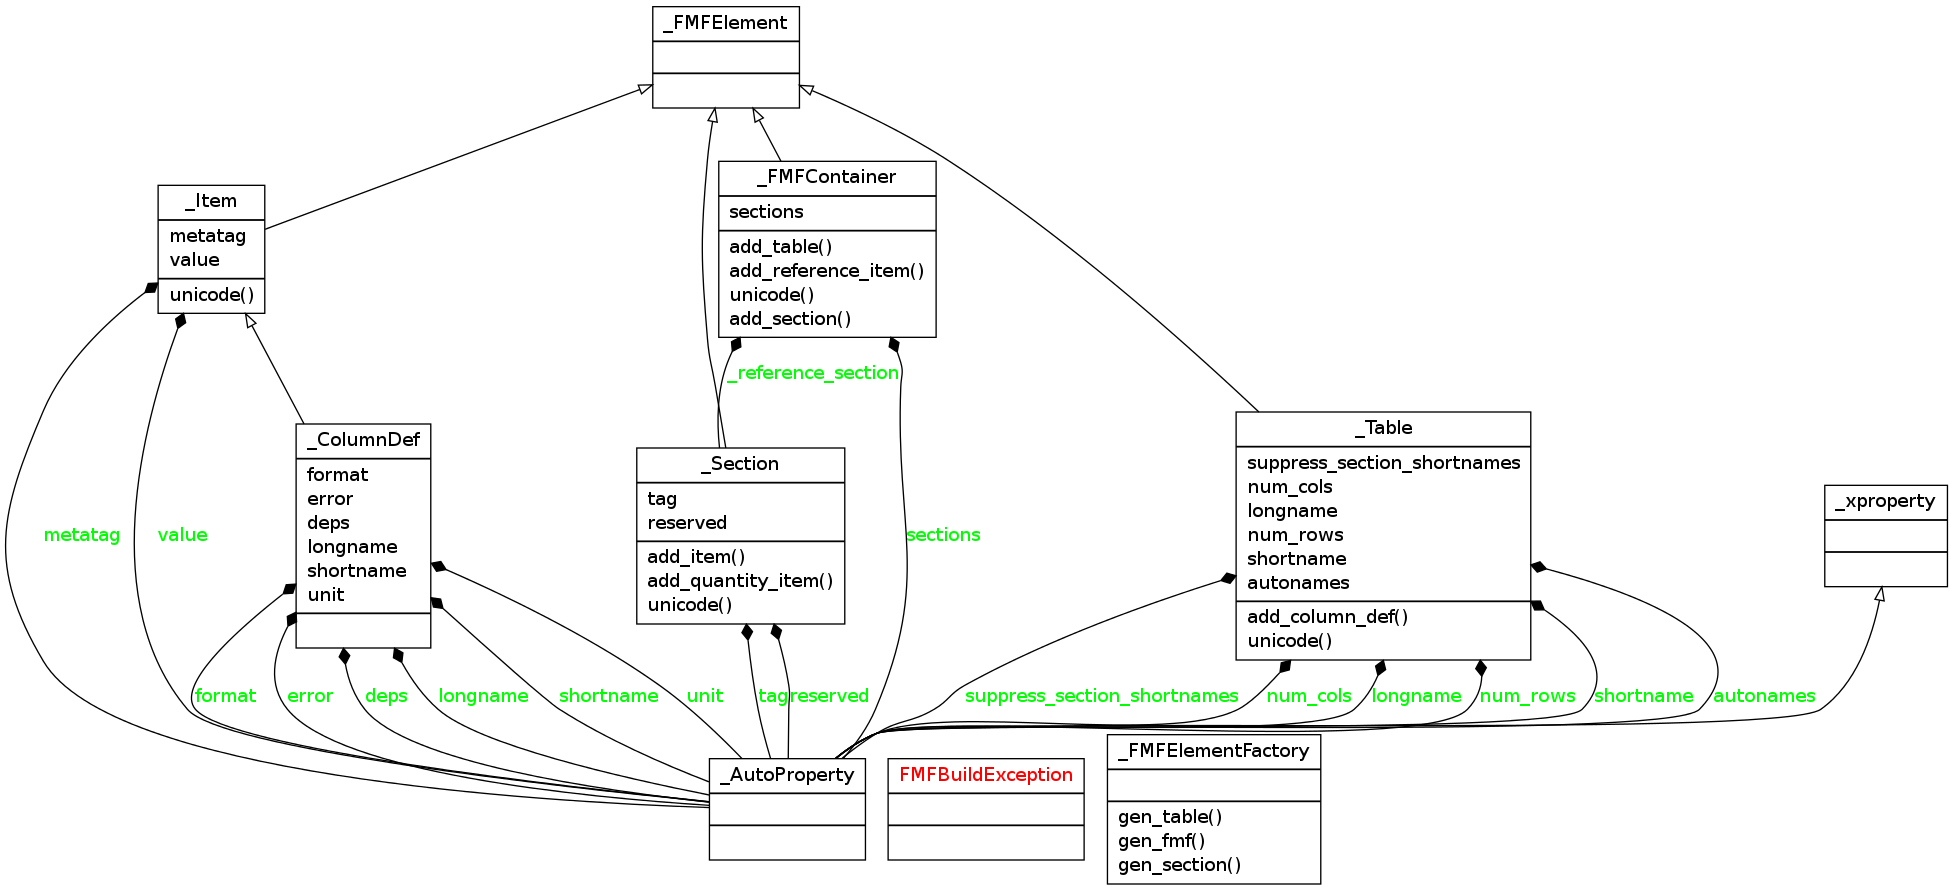
\includegraphics[width=\textwidth]{./classes_pyphant_fmf}
\caption{The class diagram of the FMF implementation that is part of the Pyphant data analysis software. Class diagram generated by \enquote{pyrevert}.}
\label{fig:classes_pyphant_fmf}
\end{sidewaysfigure}

The functionality of Pyphant roots in data structures that are derived from the base class \enquote{DataContainer}. This includes the above mentioned \enquote{FieldContainer} as well as an object called \enquote{SampleContainer} that will not be further discussed here. These data structures embody a philosophy similar to the FMF: To keep data, units and errors together and enable simultaneous processing as well as keeping metadata in the same data structure with data.

Thus, a \enquote{Field Container} (FC) holds data similar to a typical FMF of a measurement: The object called \enquote{data} in an FC holds one dimensional data that can depend on an arbitrary number of \enquote{axes}. The FC aditionally may hold the physical unit of the data and an error as well as a dictionary of parameters. The axes themselves are one dimensional FCs. Every FC has a longname and a shortname. As the axes are FC, this holds also true for them. For information about the \enquote{DataContainer} and \enquote{FieldContainer} classes including attributes, see Figure \ref{fig:class_field_container}.\\

\begin{figure}
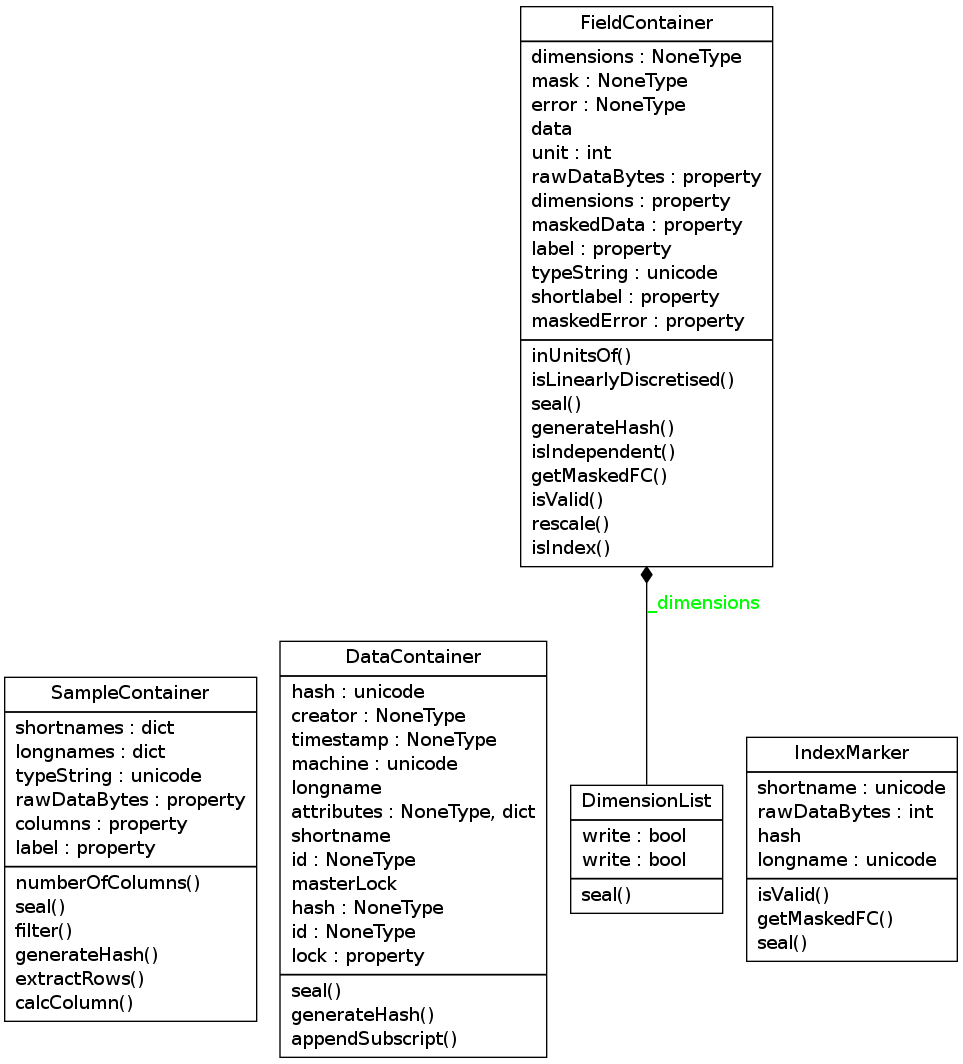
\includegraphics[width=\textwidth]{./classes_data_containers}
\caption{The \enquote{FieldContainer} class in Pyphant. The \enquote{dimensions} attribute holds the axes, the \enquote{error} holds the error data, \enquote{data} holds the data and \enquote{unit} the unit of data and error. \enquote{longname} and \enquote{shortname} are attributes of the \enquote{DataContainer} class from which \enquote{FieldContainer} inherits. Note that the \enquote{DataContainer} class has a \enquote{creator}, \enquote{timestamp} and \enquote{machine} attribute, too. These attributes hold information which can be used to generate a \enquote{*reference} section. Further parameters are held in the \enquote{attributes} attribute of the \enquote{DataContainer} class.}
\label{fig:class_field_container}
\end{figure}

During the generation of an FMF instance from a FC in Pyphant, the axes, the data and the error are interpreted as columns of a table. The longnames of the axes are used as names of the according columns in the data definitions. The shortnames of the axes constitute the according symbols, together with units if there are any. The name of the column holding the one dimensional \enquote{data} from the FC in the data definitions is the longname of the FC. The according  symbol is composed of the FCs shortname, the known dependencies on the axes, the unit and the symbol of the error column if given. Name and symbol of the column holding the error are also derived from the original FCs long- and shortname.

\section{APPENDIX III: Rudimentary implementations in python: readfmf and simplefmf}

There are already two rudimentary implementations of FMF as stand-alone libraries in phyton: readfmf and simplefmf. While read\-fmf is a implementation for reading FMF files, simplefmf is an implementation for writing. Both are available on GitHub.
%\href{https://github.com/SGWissInfo/readfmf}{readfmf}; \href{https://github.com/SGWissInfo/simplefmf}{simplefmf}

\subsection{readfmf}

readfmf is derived from pythons \enquote{ConfigObj}. Calling the function \fcal{stream2data}{filepointer} returns two objects, representing the FMF data from the stream indicated by \textit{filepointer}. The first of the two returned objects is of type \enquote{ConfigObj} and contains a dict holding the data from the meta sections. The second returned object is of type \enquote{ndarray} and contains the data of the tables, indexed by the table symbol and ordered in column, row as string values. There are \emph{no} CL or version checks.

\subsection{simplefmf}

simplefmf comprises three individual classes, \enquote{FMFDataDefinition}, \enquote{FMFTable} and \enquote{SimpleFMF}, the former two aggregated to the latter that represents the FMF. \enquote{FMFDataDefinition} handles the data definitions for the \enquote{FMFTable} objects. The meta sections are stored and handled within the \enquote{SimpleFMF} object. The entries of the meta sections, as well as the table definitions are stored as key-value pairs of strings. Table data are stored in their respective types and a formatter can be choosen for output. Thus \enquote{simplefmf} resembles CL 1 without reflecting the API defined above.

\bibliography{./fmf_references}
\bibliographystyle{plain}

\end{document}